\documentclass[12pt,english]{article}

\usepackage{natbib}

\usepackage{graphics,graphicx,dcolumn,bm,fleqn,epic,eepic,float}
\usepackage{amssymb,amsmath,multirow,rotate,rotating,color}
\usepackage[utf8]{inputenc}

\usepackage[english]{babel}
\usepackage{caption}
\usepackage{subcaption}
\usepackage{tikz}
\usepackage{hyperref}
\hypersetup{
    colorlinks=true,
    linkcolor=blue,
    filecolor=magenta,      
    urlcolor=cyan,
}
%\usepackage[usenames,dvipsnames,svgnames,table]{xcolor}
\tikzset{fontscale/.style = {font=\relsize{#1}}}
\usetikzlibrary{calc}
\makeatother

\newcommand{\figref}[1]{Fig.~\ref{fig:#1}}
\newcommand{\eqnref}[1]{Eq.~(\ref{eq:#1})}
\newcommand{\ts}{\textsuperscript}

\definecolor{tuered}{RGB}{214,0,74}

\newcommand{\todo}[1]{\textbf{\textcolor{tuered}{ TODO: #1}}}

\newcommand{\vectornorm}[1]{\left|\left|#1\right|\right|}

\renewcommand{\vec}[1]{\mathbf{#1}}
\newcommand{\uvec}[1]{\hat{\vec{#1}}}
\newcommand{\tensor}[1]{\mathbf{#1}}

\definecolor{pyblue}{HTML}{1F77B4}
\definecolor{pyorange}{HTML}{FF7F0C}
\definecolor{pygreen}{HTML}{2CA02C}
\definecolor{pyred}{HTML}{D62728}

\newcommand{\JH}[1]{\textcolor{blue}{JH: #1}}
\begin{document}

% The referee PDF has been generated from r239 -- 'make referee' command.


\section*{Reply to Referee B}

We thank the Referee for his/her thorough reading of our manuscript and detailed report.
We are happy to read that the referee acknowledges the amount of work we did and thinks it could be fitting for PRL after revision.
In what follows we provide detailed answers to all Referee's questions and we discuss all the changes made to the manuscript
(which are typeset in red color).

\begin{itemize}


\item[ \textbf{\underline{Comment 1.}}]
{
The model disjoining pressure, Eq. 3 with a tail decaying as the
inverse squared power seems odd. I am more familiar with the expected
van der Waals tail with a decay as the inverse cube power. Is there
any reason for this choice?

\item[ \textbf{Answer}]
{
The Referee is right in pointing out that, indeed, the $h^{-3}$ decay 
for the attractive part of the disjoining pressure is more straightforward 
to understand as it can be derived directly from an intermolecular potential of Lennard-Jones type. Nevertheless, it is also true that other forms
can be encountered in the literature, depending on the actual interactions
\cite{SCHWARTZ1998173,Mitlin,Teletzke}. Here, though, our choice of the $(3,2)$ pair of exponents is motivated more by computational reasons rather than by the will of 
simulating a specific liquid with given physical properties.
With such choice, in fact, the characteristic dewetting time 
is shorter, thus making the overall computational cost more manageable.
In fact, we have seen in a previous study~\cite{PhysRevE.104.034801} that,
except for this shift of the time scales, the dewetting dynamics remains 
qualitatively the same. To confirm this observation, we have run 
a new simulation (for a single pair of pattern wavelength and speed) 
with the $(9,3)$ exponents and show the results in figure \ref{fig:rivulets_9_3} of this reply.
\begin{figure}
    \centering
    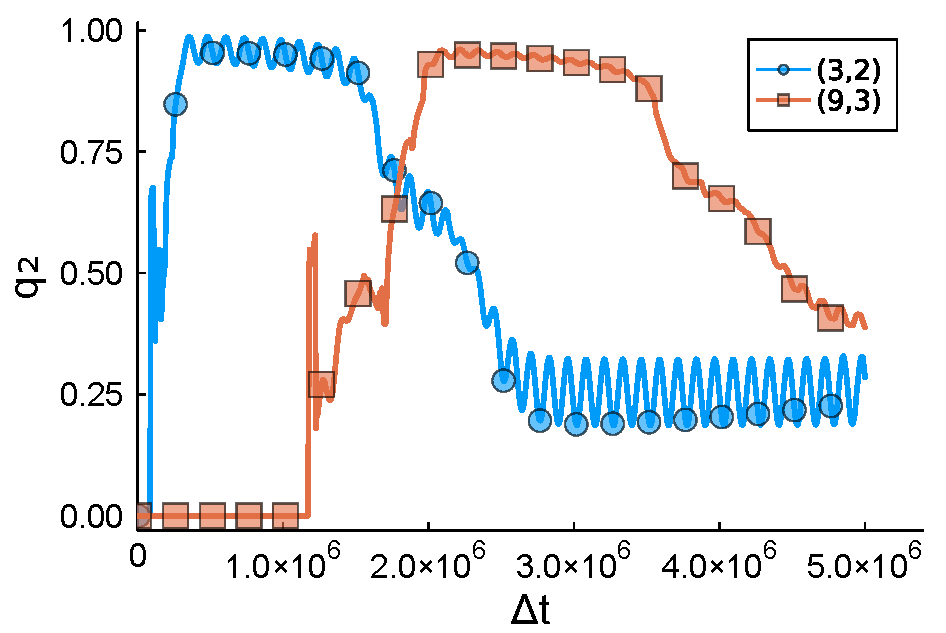
\includegraphics[width=0.7\textwidth]{refBFig_1.pdf}
    \caption{Minkowski metric $q_2$ as a function of time for 
    $\Gamma = 1.5$ and $\lambda = 256 h_0$ from two simulations with different disjoining 
    pressure exponents, $(9,3)$ and $(3,2)$ (as in the paper) respectively.}
    \label{fig:rivulets_9_3}
\end{figure}
We have added the following footnote in the paper commenting on this aspect:\\
\\
\textcolor{red}{Expressions of 
the general form $\Pi(h) = \gamma(1-\cos \theta)(n-1)(m-1)/(n-m)((h_{\ast}/h)^n - (h_{\ast}/h)^m)/h_{\ast}$
are frequently found in the literature, with various combination of exponents $(n,m)$ ($n>m$), depending
on the type of interactions among fluid molecules and between fluid and substrate~\cite{SCHWARTZ1998173,Mitlin,Teletzke}. A common choice, for instance, is the pair $(9,3)$, which 
can be derived from molecular interactions of Lennard-Jones type. Here, the use of the $(3,2)$ pair is motivated mainly by the computational advantage of keeping the characteristic dewetting time 
shorter. We have run also a single case ($\lambda=256 h_0$ and $\Gamma=1.5$) with $(9,3)$ and observed that 
the dynamics remains essentially the same, but for a shift in the time scale (see also~\cite{PhysRevE.104.034801}).}
}

\item[ \textbf{\underline{Comment 2.}}]
The second major concern refers to the choice of slip length. 
The authors study a fluid-substrate model that has a thin film equilibrium thickness of 
$0.07$ length units, but the slip length is one unit, hence about $10$ times larger than the equilibrium film thickness. 
This seems unexpected, in view of the small contact angle chosen for the system. 
Could the authors justify this choice?
}

\item[ \textbf{Answer}]
{
As the Referee correctly remarks, indeed small contact angles are typically associated to small slip lengths. From a phenomenological point of view, 
though, having $\delta \sim h_0$ is still commonly considered in the weak/intermediate slip regime, as proven, for instance, 
by the formation of satellite 
droplets following rivulet breakup~\cite{peschka2019signatures} or 
in the rim shape in dewetting by hole nucleation~\cite{fetzer2007quantifying, munch2005lubrication} (see also Fig.~\ref{fig:slip}).
\begin{figure}
    \centering
    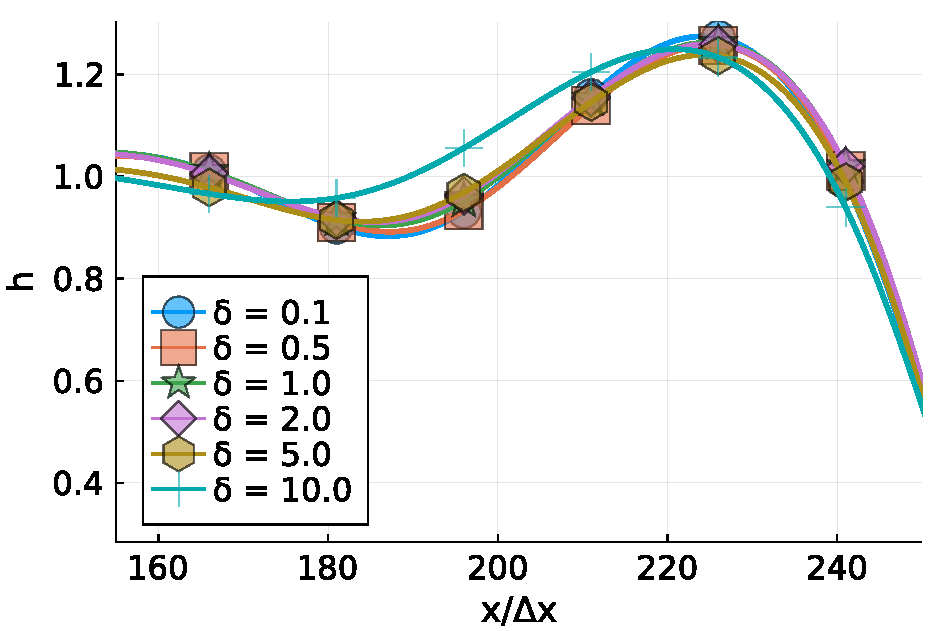
\includegraphics [width=0.6\textwidth]{refBFig_2.pdf}
    \caption{Dewetting rim profiles for various slip parameters $\delta$; notice the presence of a dimple behind the front, typical of 
    small to vanishing slip, which is preserved for slip lengths up to 
    $\delta \sim 10 h_0$.}
    \label{fig:slip}
\end{figure}
Our choice of this slip length value was dictated essentially by the need 
to keep numerical stability even in the strongly time dependent case 
(large pattern speed), yet remaining in a small slip regime. 
Nevertheless, motivated by the Referee's concern and in order to check that 
picture remains qualitatively the same, we have run a simulation with 
a slip length four times smaller. The results from the analysis of the Minkowski metric $q_2$, for two cases with low and high pattern speed, reveal that indeed
the droplet-to-rivulet transition is confirmed, with $\Gamma$ as the 
discriminating parameter (see figure \ref{fig:q2smallslip}).
\begin{figure}
    \centering
    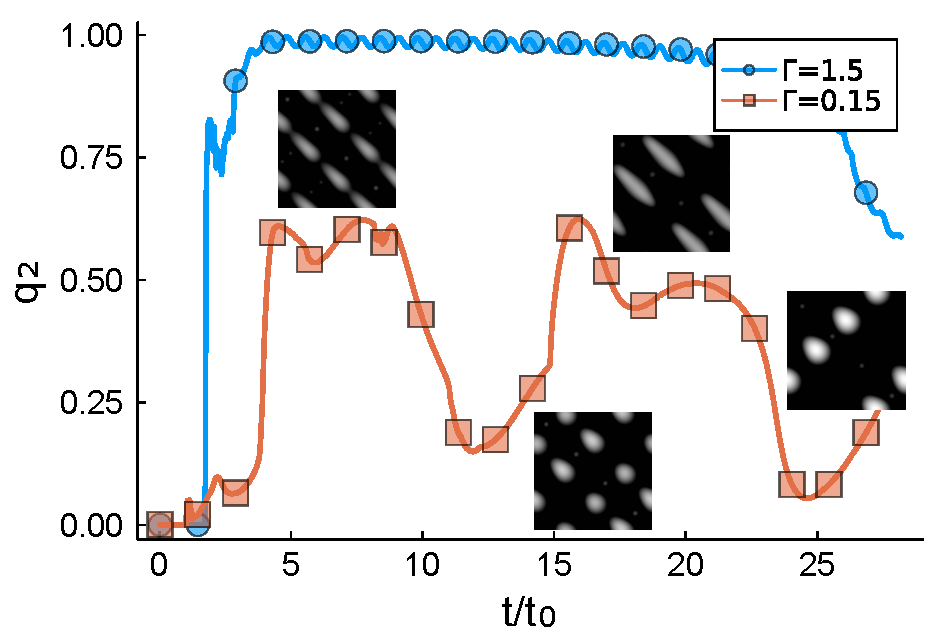
\includegraphics [width=0.75\textwidth]{refBFig_3.pdf}
    \caption{Minkowski metric $q_2$ as a function of time for two pattern speeds and slip velocity $\delta = 0.25 h_0$, signalling that the emergence of rivulets for $\Gamma>1$
    is preserved.}
    \label{fig:q2smallslip}
\end{figure}
We have commented on this when we give the value of the slip length, saying that:\\
\\
\textcolor{red}{To regularize the contact line divergence~\cite{huh1971hydrodynamic} we use a precursor layer thickness $h_{\ast}/h_0=0.07$ and a slip length $\delta/h_0 = 1$, 
a value which lies
within the weak/intermediate slip regime~\cite{peschka2019signatures,fetzer2007quantifying, munch2005lubrication} (we have tried also a value four times smaller, without observing 
any major qualitative change in the results).} 
}

\item[ \textbf{\underline{Comment 3.}}]
{
The relevance of the manuscript relies on the significance of the substrate's switchable properties. 
Particularly, it is assumed that the wetting properties can be modulated on space but also on time. 
The authors have mentioned in the introduction that this can be potentially done. 
However, it would be desirable that the authors relate their model of switchable substrate with some specific experimental realization, where the actual length and time scales are mentioned.
}

\item[ \textbf{{Answer}}]
{
%This is indeed a very interesting comment.
%Although our approach, as theorists/numericists, can be seen more of {\it theoretical
%engineering} and our picture would be, then, unlikely devoid of flaws, we are glad 
%to try to envisage a potential experiment.
%\JH{??}
%We thank the Referee for bringing this up.
%First, we like to note that experiments are not our field of expertise and therefore %our envisioned realization could be flawed.
%The two relevant scales are $t_0$ and $q_0$ (or $2\pi/q_0$).
%Considering the experimental parameters from~\cite{becker2003complex,PhysRevLett.99.114503} %we get, 
%\begin{align*}
%    t_0 &\approx 300\,\text{s},\qquad~~~\qquad \frac{2\pi}{q_0}\approx 
%    400\,\text{nm}.
%\end{align*}
%The time scale is in the region of minutes and the wettability pattern wavelengths are %in the interval $(800\,\text{nm}, 4000\,\text{nm})$. 
A possibility could be to prepare a thin liquid film on a light responsive substrate~\cite{IchimuraEtAl_Science2000}, under the action of controlled 
external stimuli (a light emitter). 

\textcolor{red}{An ideal candidate could be a digital multimirror device (DMD).
This technology has effectively been used for thin film experiments and additive manufacturing~\cite{doi:10.1021/jp301092y, doi:10.1126/science.aax8760}, it allows for fast temporal modulations of the optical signal (with frequencies up to $\approx 16 \, \text{kHz}$)
with spatial resolution of $\approx 10 \times 10 \, \mu \text{m}^2$ (the size of a pixel).
Considering as a reference, for instance, the system studied in ~\cite{becker2003complex,PhysRevLett.99.114503}, namely a $\sim 4 \, \text{nm}$ thick film 
of polystyrene deposited on an oxidized silicon wafer,  
we evaluate the retraction speed 
$U_{\Theta} = \frac{\Theta^3 \gamma}{9 \mu}$ to be 
$U_{\Theta} \approx 10^{-2} \, \mu \text{m}/\text{s}$. 
The (minimum) {\it pattern speed} can be 
estimated, from the pixel size with frame rate $\sim 1 s^{-1}$, as 
$v_{\theta} \sim 10 \, \mu \text{m}/\text{s}$, that would give $\Gamma \sim 10^3$, i.e. well within 
the rivulet regime ($\Gamma > 1$). We note, also, that both $U_{\Theta}$ and $v_{\theta}$ can 
be widely modulated: the former, playing either with the (temperature and molecular weight dependent) viscosity 
or tailoring the substrate to making it more hydrophobic (i.e. increasing the contact angle); the latter, tuning
the spatial resolution and frame rate of the DMD. We expect, thus, the range of achievable $\Gamma$'s to 
be feasibly extended both to very high ($\Gamma \gg 1$) and very low ($\Gamma \ll 1$) values.} 

We have included these comments in the revised manuscript just before the conclusions.

}

\item[ \textbf{\underline{Comment 4.}}]
{
An important parameter in the problem is the wave-vector $q_0$, which sets the correlation length in the problem. 
The authors should state what the actual value is relative to either the average film height, or the wave-length of modulations. 
Is there any reason to give the wave-length of modulations in units of the system size, i.e., are the results subject to finite size effects? Otherwise it appears more meaningful to describe the modulations in units of $q_0$ or the equilibrium film thickness.
}

\item[ \textbf{{Answer}}]
{
We apologize for not giving the value of $q_0 \approx 0.09$ (corresponding to an intrinsic correlation length 
$\lambda_s = 2\pi/q_0 \approx 70 h_0$), which is now provided in the revised manuscript. We also acknowledge that expressing the wavelength in terms of the size $L$
was not at all meaningful (no finite size effects are involved). In fact, all the lengths (including $L$) are expressed in units of the mean film thickness $h_0$ (and it was so also in the old version of the paper, as commented in the text below eq. (4)). In order to avoid any confusion, we explicitly write 
the values of all lengths in terms of $h_0$ in the revised version.
}

\item[ \textbf{\underline{Comment 5.}}]
{
The thin film equation relies on a local approximation for the interface potential and disjoining pressure. 
Notice that to first order in non-local effects, the surface tension entering the thin film equation adopts a film thickness dependence which could potentially affect the dynamics. 
Particularly, as far as the parallel correlation length $q_0$ is referred, the non-local effects provide an upper bound equal to the inverse bulk correlation length. 
This could be a significant effect in polymer thin films (c.f. Benet et al. jpc-c 118, 22079, 2014 and the related discussion on dynamical effects Pahlavan et al., jfm, 845, 642, 2018).
}

\item[ \textbf{{Answer}}]
{
We guess that the Referee mentions the fact that the Laplacian of the thickness field, $\nabla^2 h$,
is just a small gradient approximation of the actual local curvature, such that the Laplace contribution to the film pressure should indeed read $\gamma \nabla^2 h/\sqrt{1+|\nabla h|^2}$. This is of course correct, but 
the condition $|\nabla h| \ll 1$ holds true in our system, owing to the very same lubrication approximation,
or, equivalently, to the small contact angles involved; the spinodal wavelength for a homogeneous substrate with
contact angle $\theta_0$ is $\lambda_s = 2\pi/q_0(\theta_0) \approx 70 h_0$. Therefore, the typical gradients
of the thickness field can be estimated as $|\nabla h| \sim h_0/\lambda_s \approx 1/70 \ll 1$ (notice 
that this is, somehow, a worst case scenario since, as we discuss in the text, in the patterned substrates
$\lambda \stackrel{>}{\sim} \lambda_s$).
We have added the following footnote, where we introduce the film pressure:\\
\\
\textcolor{red}{The Laplace pressure is the product of the surface tension 
and the local curvature, therefore its full expression reads $p_L = -\gamma \nabla^2 h/\sqrt{1+|\nabla h|^2}$; 
since we are in the lubrication regime, though, whereby $|\nabla h| \ll 1$, the denominator can be safely neglected 
and the pressure reduces to the form involving only the Laplacian of the thickness field~\cite{Benet2014,juanes2018}}, \\
\\
citing the related papers as a reference.
}
\end{itemize}


\bibliographystyle{abbrv}
\bibliography{Ref}

\end{document}
